%%
% This is an Overleaf template for presentations
% using the TUM Corporate Desing https://www.tum.de/cd
%
% For further details on how to use the template, take a look at our
% GitLab repository and browse through our test documents
% https://gitlab.lrz.de/latex4ei/tum-templates.
%
% The tumbeamer class is based on the beamer class.
% If you need further customization please consult the beamer class guide
% https://ctan.org/pkg/beamer.
% Additional class options are passed down to the base class.
%
% If you encounter any bugs or undesired behaviour, please raise an issue
% in our GitLab repository
% https://gitlab.lrz.de/latex4ei/tum-templates/issues
% and provide a description and minimal working example of your problem.
%%

\PassOptionsToClass{onlytextwidth}{beamer}

\documentclass[
  german,            % define the document language (english, german)
  aspectratio=169,    % define the aspect ratio (169, 43)
  % handout=2on1,       % create handout with multiple slides (2on1, 4on1)
  % partpage=false,     % insert page at beginning of parts (true, false)
  % sectionpage=true,   % insert page at beginning of sections (true, false)
]{tumbeamer}


% load additional packages
\usepackage{booktabs}
\usepackage{graphicx}
\usepackage{tikz}
\usepackage{url}
\usepackage{pgfplots}
\usepackage{hyperref}
\usepackage{pmboxdraw}
\usepackage{float}
\usepackage{babel}[ngerman]
\usepackage{csquotes}[autostyle]
\usepackage[useregional]{datetime2}
\usepackage{siunitx}

% tikz  
\usetikzlibrary{fit, matrix, calc, arrows, arrows.meta, positioning}

% xcolor
\definecolor{altblue}{HTML}{44C8F5}
\definecolor{altyellow}{HTML}{FFE600}
\definecolor{altgreen}{HTML}{26E600}
\definecolor{altmagenta}{HTML}{EC008C}

\captionsetup{labelformat=empty}

% image path
\graphicspath{ {./resources/} }

% beamer
\setbeamercolor{footnote}{fg=black}
\setbeamercolor{footnote mark}{fg=black}
\renewcommand{\thempfootnote}{\arabic{mpfootnote}}

% presentation metadata
\title{Übung 02: RISC-V Assembly}
\subtitle{Einführung in die Rechnerarchitektur}
\author{Niklas Ladurner}

\institute{\theChairName\\\theDepartmentName\\\theUniversityName}
\date{\DTMdisplaydate{2024}{10}{24}{-1}}

\footline{\insertauthor~|~\insertshorttitle~|~\insertshortdate}


% macro to configure the style of the presentation
\TUMbeamersetup{
  title page = TUM tower,         % style of the title page
  part page = TUM toc,            % style of part pages
  section page = TUM toc,         % style of section pages
  content page = TUM more space,  % style of normal content pages
  tower scale = 1.0,              % scaling factor of TUM tower (if used)
  headline = TUM threeliner,      % which variation of headline to use
  footline = TUM default,         % which variation of footline to use
  % configure on which pages headlines and footlines should be printed
  headline on = {title page},
  footline on = {every page, title page=false},
}

% available frame styles for title page, part page, and section page:
% TUM default, TUM tower, TUM centered,
% TUM blue default, TUM blue tower, TUM blue centered,
% TUM shaded default, TUM shaded tower, TUM shaded centered,
% TUM flags
%
% additional frame styles for part page and section page:
% TUM toc
%
% available frame styles for content pages:
% TUM default, TUM more space
%
% available headline options:
% TUM empty, TUM oneliner, TUM twoliner, TUM threeliner, TUM logothreeliner
%
% available footline options:
% TUM empty, TUM default, TUM infoline


\begin{document}

\maketitle

\begin{frame}[c]{}{}
	\begin{center}
		\LARGE  Keine Garantie für die Richtigkeit der Tutorfolien.

		\Large Bei Unklarheiten/Unstimmigkeiten haben VL/ZÜ-Folien recht!
	\end{center}
\end{frame}

\begin{frame}[c]{Abstraktionsebenen}{}
	\begin{columns}[c]
		\begin{column}{0.6\textwidth}
			\begin{itemize}
				\item Code in einer Hochsprache (C, Java\footnote{im Regelfall zu Bytecode kompiliert}, \textellipsis) ist lediglich eine Abstraktion
				\item Compiler: Hochsprache $\rightarrow$ Assemblercode
				\item Assembler: Assemblercode $\rightarrow$ Maschinencode\\(1:1 Übersetzung)
				\item Maschinencode ist plattformspezifisch!
				\item ISA: \enquote{Bedienungsanleitung} einer CPU
				      %        \item RISC vs. CISC
			\end{itemize}
		\end{column}
		\begin{column}{0.3\textwidth}
			\begin{figure}
				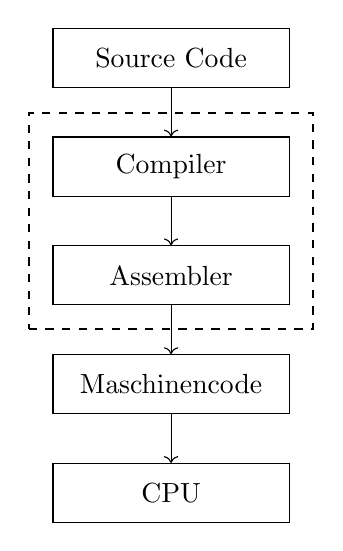
\begin{tikzpicture}[
						block/.style = {draw, rectangle, minimum width=3cm, minimum height=0.75cm, align=center},
						node distance=1.2cm
					]

					\node[block] (source) at (0,0) {Source Code};
					\node[block, yshift=-1cm] (compiler)  at (source.south){Compiler};
					\node[block, yshift=-1cm] (assembler) at (compiler.south){Assembler};
					\node[block, yshift=-1cm] (machine) at (assembler.south) {Maschinencode};
					\node[block, yshift=-1cm] (cpu) at (machine.south) {CPU};

					\draw[->] (source) -- (compiler) node[midway, right] {};
					\draw[->] (compiler) -- (assembler) node[midway, right] {};
					\draw[->] (assembler) -- (machine) node[midway, right] {};
					\draw[->] (machine) -- (cpu) node[midway, right] {};

					\node[draw, dashed, thick, inner sep=0.3cm, fit=(compiler) (assembler)] {};
				\end{tikzpicture}
				\footnotesize  (Abbildung stark vereinfacht)
			\end{figure}
		\end{column}
	\end{columns}
	\setcounter{footnote}{1}
\end{frame}

\begin{frame}[c]{RISC vs. CISC}{}
	\begin{columns}
		\begin{column}{0.5\textwidth}
			\centering\textbf{R}educed \textbf{I}nstruction \textbf{S}et \textbf{C}omputer
			\vspace{0.5\baselineskip}
			\begin{itemize}
				\item beschränkte Menge an Instruktionen
				\item einfache Implementierung, schnelle Dekodierung
				\item komplexere Operationen benötigen mehrere Instruktionen
			\end{itemize}
			\vspace{0.5\baselineskip}
			Beispiel: RISC-V
		\end{column}
		\begin{column}{0.5\textwidth}
			\centering\textbf{C}omplex \textbf{I}nstruction \textbf{S}et \textbf{C}omputer
			\vspace{0.5\baselineskip}
			\begin{itemize}
				\item mächtiges Instruktionsset
				\item komplexe Implementierung, Realisierung als Mikrocode, langsame Dekodierung
				\item dedizierte Instruktion für beinahe jede Operation\footnote[frame]{am Beispiel x86: \href{https://www.felixcloutier.com/x86/vcvttps2uqq}{\texttt{VCVTTPS2UQQ}}, \href{https://www.felixcloutier.com/x86/gf2p8affineinvqb}{\texttt{GF2P8AFFINEINVQB}}, \href{https://www.felixcloutier.com/x86/maskmovdqu}{\texttt{MASKMOVDQU}} :)}
			\end{itemize}
			\vspace{0.5\baselineskip}
			Beispiel: x86-64
		\end{column}
	\end{columns}
\end{frame}

\begin{frame}[c]{RISC-V}{}
	\begin{columns}[c]
		\begin{column}{0.7\textwidth}
			\begin{itemize}
				\item Befehlssatz in ERA: RV32IM
				\item 32 Register, einige davon mit spezieller Funktion
				\item Instruktionen auf 32 Bit begrenzt
				      \\$\rightarrow$ Konstanten müssen zusammengebastelt werden
				\item Datenwortbreite: 32 Bit (4 Byte)
				\item Little-Endian-Architektur
				\item Byte-adressierbarer Speicher, maximale Hauptspeichergröße?
				      \visible<2->{\\$\rightarrow$ $2^{32}$ Adressen, ca. \qty{4.3}{\giga\byte}}
			\end{itemize}
		\end{column}
		\begin{column}{0.3\textwidth}
			
\includegraphics[width=\linewidth]{w02_risc_v_logo.png}
		\end{column}
	\end{columns}
\end{frame}

\begin{frame}[c]{Register}{}
	\begin{center}
		{\rmfamily
			\begin{tabular}{|l|l|l|c|}
				\hline
				Register        & ABI Name       & Description                      & Saver\footnote{Erst in zwei Wochen relevant} \\ \hline
				\texttt{x0}     & \texttt{zero}  & Hard-wired zero                  & ---                                          \\
				\rowcolor{altblue}
				\texttt{x1}     & \texttt{ra}    & Return address                   & Caller                                       \\
				\texttt{x2}     & \texttt{sp}    & Stack pointer                    & Callee                                       \\
				\texttt{x3}     & \texttt{gp}    & Global pointer                   & ---                                          \\
				\texttt{x4}     & \texttt{tp}    & Thread pointer                   & ---                                          \\
				\texttt{x5-x7}  & \texttt{t0-t2} & Temporaries                      & Caller                                       \\
				\texttt{x8}     & \texttt{s0/fp} & Saved register/frame pointer     & Callee                                       \\
				\texttt{x9}     & \texttt{s1}    & Saved register                   & Callee                                       \\
				\rowcolor{altyellow}
				\texttt{x10-11} & \texttt{a0-1}  & Function arguments/return values & Caller                                       \\
				\texttt{x12-17} & \texttt{a2-7}  & Function arguments               & Caller                                       \\
				\rowcolor{altmagenta}
				\texttt{x18-27} & \texttt{s2-11} & Saved registers                  & Callee                                       \\
				\rowcolor{altgreen}
				\texttt{x28-31} & \texttt{t3-6}  & Temporaries                      & Caller                                       \\ \hline
			\end{tabular}
		}
	\end{center}
\end{frame}

\begin{frame}[c]{Immediates}{}
	\begin{columns}[c]
		\begin{column}{0.5\textwidth}
			\begin{itemize}
				\item als \enquote{Konstanten} in Instruktion enkodiert
				\item RV32IM verwendet 12- und 20-Bit Immediates
				\item Datenwortbreite 32 Bit $\rightarrow$ \enquote{Erweiterung} von Immediates notwendig
				\item Sign- vs. Zero-Extension
				\item Achtung: Immediates werden immer als signed Zahlen interpretiert!
			\end{itemize}
		\end{column}
		\begin{column}{0.5\textwidth}
			\begin{center}
				%				\includegraphics[width=0.75\textwidth]{asm_signext.pdf}
				\begin{figure}
					\begin{tikzpicture}
						\def\sz{1.75em}
						\def\brpad{3.25ex}

						\tikzset{
							lbl/.style={draw=none, minimum width=\sz, minimum height=\sz, text depth=1pt},
							attr/.style={draw, minimum width=\sz, minimum height=\sz, inner sep=0pt, text width=\sz, anchor=center, align=center},
							mat/.style={matrix of nodes, ampersand replacement=\&, nodes={attr}, row sep=1.5em, column sep=-\pgflinewidth},
							br/.style={decorate,decoration={brace, amplitude=1ex, raise=0.5ex}},
							brinv/.style={br,decoration={mirror}},
							arrow/.style={latex-},
						}



						\matrix[mat] (m1) {
							\textcolor{TUMBlue}{0}\&\textcolor{TUMBlue}{0}\&\textcolor{TUMBlue}{\textellipsis}\&\textcolor{TUMBlue}{0}\&\textcolor{TUMBlue}{0}\&\textcolor{TUMBlue}{0}\&1\&\textellipsis\&1\&1\&0%
							\\
						};

						%		\node[attr, thick] at (m1-1-6) {};


						\matrix[mat, below=1.75cm of m1] (m2) {
							\textcolor{TUMBlue}{1}\&\textcolor{TUMBlue}{1}\&\textcolor{TUMBlue}{\textellipsis}\&\textcolor{TUMBlue}{1}\&\textcolor{TUMBlue}{1}\&\textcolor{TUMBlue}{1}\&1\&\textellipsis\&1\&1\&0%
							\\
						};

						%	\node[attr, thick] at (m2-1-6) {};

						\foreach \x in {1, 2}
							{
								\draw [br] (m\x-1-6.north west) -- (m\x-1-11.north east) node[midway, yshift=\brpad]{12 bit};

								\draw [brinv] (m\x-1-1.south west) -- (m\x-1-11.south east) node[midway, yshift=-\brpad]{32 bit};
							}

						%		\foreach \x in {1, 2, 3, 4, 5}
						%		{
						%			\draw[arrow] ($(m1-1-\x.north) + (0.05,0)$) to [out=90,in=90,looseness=2] ($(m1-1-\fpeval{\x+1}.north) + (-0.05,0)$);
						%		}
					\end{tikzpicture}
					\caption{Sign Extension}
				\end{figure}
			\end{center}
		\end{column}
	\end{columns}
\end{frame}

\begin{frame}[c]{}{}
	\begin{center}
		\LARGE Fragen?
	\end{center}
\end{frame}


\begin{frame}[fragile, c]{Links}{}
	\begin{itemize}
		\item Zulip: \href{https://zulip.in.tum.de/#narrow/channel/3255-ERA-Tutorium-.E2.80.93-Mi-1600-3}{\enquote{ERA Tutorium -- Mi-1600-3}}
		      bzw. \href{https://zulip.in.tum.de/#narrow/channel/3264-ERA-Tutorium-.E2.80.93-Fr-1500-1}{\enquote{ERA Tutorium -- Fr-1500-1}}
		\item \href{https://www.moodle.tum.de/course/view.php?id=111440}{ERA-Moodle-Kurs}
		\item \href{https://artemis.in.tum.de/courses/516}{ERA-Artemis-Kurs}
		\item \href{https://vanhunteradams.com/FixedPoint/FixedPoint.html}{Einführung Fixpunktarithmetik}, \href{https://specbranch.com/posts/fixed-point/}{Alternative}
		\item \href{https://msyksphinz-self.github.io/riscv-isadoc/html/index.html}{Übersicht an RISC-V-Instruktionen}
	\end{itemize}
\end{frame}

\maketitle

\end{document}
